\documentclass[12pt,twoside]{article}

\usepackage{paperlighter}

% Recommended, but optional, packages for figures and better typesetting:
\usepackage{microtype}
\usepackage{graphicx}
\usepackage{subfigure}
\usepackage{booktabs} % for professional tables

% Attempt to make hyperref and algorithmic work together better:
\newcommand{\theHalgorithm}{\arabic{algorithm}}


% For theorems and such
\usepackage{amsmath}
\usepackage{amssymb}
\usepackage{mathtools}
\usepackage{amsthm}

% if you use cleveref..
\usepackage[capitalize,noabbrev]{cleveref}

%%%%%%%%%%%%%%%%%%%%%%%%%%%%%%%%
% THEOREMS
%%%%%%%%%%%%%%%%%%%%%%%%%%%%%%%%
\theoremstyle{plain}
\newtheorem{theorem}{Theorem}[section]
\newtheorem{proposition}[theorem]{Proposition}
\newtheorem{lemma}[theorem]{Lemma}
\newtheorem{corollary}[theorem]{Corollary}
\theoremstyle{definition}
\newtheorem{definition}[theorem]{Definition}
\newtheorem{assumption}[theorem]{Assumption}
\theoremstyle{remark}
\newtheorem{remark}[theorem]{Remark}

% Todonotes is useful during development; simply uncomment the next line
%    and comment out the line below the next line to turn off comments
%\usepackage[disable,textsize=tiny]{todonotes}
\usepackage[textsize=tiny]{todonotes}



\slimtitle{Route Planning}
\slimauthor{Yijie LUO}


\begin{document}

\lightertitle{Route Planning - DS Final Project 2022 Spring}
\lighterauthor{Yijie LUO, SJTU ID 519260910009}

% \lighteraddress{$^\dagger$}{Address One}
% \lighteraddress{$^\ddagger$}{Address Two}

\lighteremail{excespo@sjtu.edu.cn}

% py: \mintinline{c++}{std::cout(x**2)}
% \mint{python}|import this|
\quad \mintinline{python}{ }
% \setcounter{section}{-1}
\begin{abstract}
In this project for final of SPEIT's data structure 2022 spring lesson, I'm going to use various data structure to represent a geographic map of China, and to plan a shortest path on this map. My tool includes \verb|C++|, \verb|Make| and \verb|CMAKE|, installed with \verb|Docker|. By using adjacency representation, heap structure and finally implementing the Dijkstra algorithm, I successfully finished the tasks listed in the handout \href{https://oc.sjtu.edu.cn/courses/44241/files/4550729?module_item_id=702072}{here}.
\end{abstract}
\section{T1}

In this task, we will design AM(adjacency matrix), AL(adjacency list) and printAM, printAL

\subsection{Adjacency Matrix}
Adjacency matrix (abbreviate to AM) is a matrix where the columns and rows are the vertices of the graph, and the element of the matrix represents the adjacency condition. If we take row $i$ that represents city $A$ and column $j$ that represents city $B$ as example, the AM is written as \verb|adjMat|.
\begin{itemize}
    \item The item $\text{adjMat}_{i, j}$ =  - \verb|INF|, if the city $A$ and $B$ is not adjacent. As there is no direct route between $A$ and $B$, we set the distance to negative infinity to represent the inaccessibility.
    \item The item $\text{adjMat}_{i, j} = d \geq 0$, in this case the cities are adjacent and the distance of the direct route is $d$. (Notice that the distance is always not negative)
\end{itemize}
We also notice that if $i=j$, $A$, $B$ is the same city, then $d = 0$. Also we have $\text{adjMat}_{i, j} = \text{adjMat}_{j, i}$, as the route is always bidirectional. We conclude that the AM is always a symmetric matrix with non-negative items.

In this situation, we first define the basic types for ou data, including vertices and edges.

\begin{minted}[mathescape, linenos, numbersep=5pt, gobble=2, frame=lines, framesep=2mm]{c++}
    /* include/types.h */
    using vertice_type = std::string;
    using edge_type = std::pair<vertice_type, vertice_type>;
    using weighted_edge_type = std::pair<edge_type, int>;
\end{minted}

\subsubsection*{a. implement the \textbf{AM} data structure}
And we introduce the public interface of the class \verb|AdjacentMatrix|. The class maintain all the vertices in a \mintinline{c++}{std::vector<vertice_type>} container. And a bidirectional map from the vertices' names to their indices in the rows and columns of the matrix, with type \mintinline{c++}{vertice_to_idx_map_type} \newline \mintinline{c++}{ = std::map<vertice_type, int>} and type \mintinline{c++}{idx_to_vertice_map_type} \newline \mintinline{c++}{ = std::map<int, vertice_type>}. They'are quite useful when we want to convert between city names and the AM structure.

\begin{minted}[mathescape, linenos, numbersep=5pt, gobble=2, frame=lines, framesep=2mm]{c++}
    /* include/adjacency.h */
    AdjacencyMatrix(std::vector<vertice_type> vs, 
                    std::vector<weighted_edge_type> wes);
    ~AdjacencyMatrix(){};
    std::vector<vertice_type> get_vertices() { return _vertices; }
    vertice_to_idx_map_type get_v2idx() { return _v2idx; }
    idx_to_vertice_map_type get_idx2v() { return _idx2v; }
    adj_matrix_type get_adjMat() { return _adjMat; }
    int get_v_size(void) { return _v_size; }
    int get_e_size(void) { return _e_size; }
    void print();
\end{minted}

You can see that the only part to implement is the constructor of the class and the \verb|print| function. We will now explain how to constrcut with explicit arguments of all vertices and all weighted edegs(that's to say with the distances between cities). We experience three phases:

\begin{itemize}
    \item With all vertices, map them to their position in the vector, and use the same position in the construction phases of the matrix
    \item Initialization phase of the matrix, the size of matrix being the number of vertices, and pad the diagonal line to $0$ (always 0 whatever the map looks like)
    \item Traverse all the weighted edges to fill the matrix. Vacant positions in the matrix we pad them with \verb|-INF| as they represent the inaccessibility.
\end{itemize}

By doing so, we successfully maintain the private variables of a vector of vertices, two maps between vertices and indices, and the matrix itself, being a two-dimensional vector.

\subsubsection*{b. Implement the generic \textbf{PrintAM} function}
As for printing the adjacent matrix, we just need to leave space for the rows and columns, and print the matrix by traversing the vector container in order, which is quite naive and simple. The result is shown below:

\begin{verbatim}
================ TEST FOR AM BEGINS ================
Our map has 13 vertices and 24 edges.
Print Adjacency Matrix:
       WL   LZ   LS   XA   CD   KM   BJ   WH   GZ   SY   TJ   SH   FZ
  WL    0  130  120    N    N    N    N    N    N    N    N    N    N
  LZ  130    0  111   84   85    N    N    N    N    N    N    N    N
  LS  120  111    0    N  110    N    N    N    N    N    N    N    N
  XA    N   84    N    0   87    N   90   94    N    N    N    N    N
  CD    N   85  110   87    0   86    N   99  102    N    N    N    N
  KM    N    N    N    N   86    0    N    N  101    N    N    N    N
  BJ    N    N    N   90    N    N    0  100    N   88    9    N    N
  WH    N    N    N   94   99    N  100    0   98    N   97   96   95
  GZ    N    N    N    N  102  101    N   98    0    N    N    N   91
  SY    N    N    N    N    N    N   88    N    N    0   89    N    N
  TJ    N    N    N    N    N    N    9   97    N   89    0   93    N
  SH    N    N    N    N    N    N    N   96    N    N   93    0   92
  FZ    N    N    N    N    N    N    N   95   91    N    N   92    0
================= TEST FOR AM ENDS =================
\end{verbatim}

Where \verb|N| is a symbol that just represents the value \verb|-INF|.

\subsection{Adjacency List}
\subsubsection*{c. Implement the \textbf{AL} data structure}
When cities are uniformly distributed geographically, it is likely that the number of edges is not much large than that of vertices (Imagine the extreme case where all vertices are connected to any other verice, and if the number of vertices is $n$, then number of edges can reach $n*(n-1)$). Therefore the AM will be sparse. 

To solve this problem, we can use a bucket to store all the neighbors of a vertice, and we store the buckets in another dimension. This is the idea of Adjacency list (abbreviate to AL) We use a vector of type \verb|vertice_type| to store one bucket, and the list node of type \verb|std::pair<vertice_type,|\newline \verb|std::vector<vertice_type>>| to store both the head vertice and its neighbor bucket. A vector of type being such node type helps us store the whole AL. 

\begin{verbatim}
    AdjacencyMatrix(std::vector<vertice_type> vs, 
                    std::vector<weighted_edge_type> wes);
    ~AdjacencyMatrix(){};
    std::vector<vertice_type> get_vertices() { return _vertices; }
    vertice_to_idx_map_type get_v2idx() { return _v2idx; }
    idx_to_vertice_map_type get_idx2v() { return _idx2v; }
    adj_matrix_type get_adjMat() { return _adjMat; }
    int get_v_size(void) { return _v_size; }
    int get_e_size(void) { return _e_size; }
    void print();
\end{verbatim}

The constructor of the AL is quite similar to that of AL.

\subsubsection*{d. Implement the generic \textbf{PrintAL} function}
We print the AL in the form given in the handout and the result is:

\begin{verbatim}
================ TEST FOR AL BEGINS ================
Our map has 13 vertices and 24 edges.
Print Adjacency List:
WL -> LZ -> LS -> N
LZ -> WL -> LS -> XA -> CD -> N
LS -> WL -> LZ -> CD -> N
XA -> LZ -> CD -> BJ -> WH -> N
CD -> LZ -> LS -> XA -> KM -> WH -> GZ -> N
KM -> CD -> GZ -> N
BJ -> XA -> WH -> SY -> TJ -> N
WH -> XA -> CD -> BJ -> GZ -> TJ -> SH -> FZ -> N
GZ -> CD -> KM -> WH -> FZ -> N
SY -> BJ -> TJ -> N
TJ -> BJ -> WH -> SY -> SH -> N
SH -> WH -> TJ -> FZ -> N
FZ -> WH -> GZ -> SH -> N
================= TEST FOR AL ENDS =================
\end{verbatim}

That's all for \textit{task 1}.
\section{T2}

\subsection{Data Preparation}
Before analysing the given map, we will first give interfaces for the map.

\subsubsection*{generation of map in \textbf{AM}}

We prepare an interface \mintinline{c++}{AM genAM();} to generate an \verb|AM| data structure from the given map. As our \verb|AM| constructor requires a vector of vertices and a vector of edges with distance(/weight), we simply construct the two vectors by pushing all vertices and weighted edges. Finally we can get the correct AM corresponding to the map given in the handout.

\subsubsection*{a. Implement the generic \textbf{GetEdgesAM}}

The function prototype should be like \mintinline{c++}{std::vector<weighted_edge_type> getEdgesAM(AM am);} in our case. To extract the edges from AM, we just need to undergo the following phases:
\begin{itemize}
    \item traverse the half matrix, and get the position where the item isn't \verb|-INF|
    \item convert from position to city names
    \item construct the edge with the names and item value being the distance(/weight)
    \item push the edge to the array to be returned.
\end{itemize}

And to better demonstrate our edges structure, we overload the \verb|operator<<| with a friend function 
\begin{minted}[mathescape, linenos, numbersep=5pt, gobble=2, frame=lines, framesep=2mm]{c++}
    /* include/types.h */
    inline std::ostream &operator<<(std::ostream &cout, 
                                    weighted_edge_type w_edge) {
        weight_type w = w_edge.second;
        vertice_type v1 = w_edge.first.first, v2 = w_edge.first.second;
        std::cout << "[" << v1 << " <--" << w << "--> " << v2 << "]";
        return std::cout;
    }  // need inline to avoid multiple definition
\end{minted}

Our \verb|GetEdgeAM| function take the given map AM as argument and give the following result:
\begin{verbatim}
============= TEST FOR getEdgeAM BEGINS =============
Got Weighted Edges in this AM:
[WL <--130--> LZ]
[WL <--120--> LS]
[LZ <--111--> LS]
[LZ <--84--> XA]
[LZ <--85--> CD]
[LS <--110--> CD]
[XA <--87--> CD]
[XA <--90--> BJ]
[XA <--94--> WH]
[CD <--86--> KM]
[CD <--99--> WH]
[CD <--102--> GZ]
[KM <--101--> GZ]
[BJ <--100--> WH]
[BJ <--88--> SY]
[BJ <--9--> TJ]
[WH <--98--> GZ]
[WH <--97--> TJ]
[WH <--96--> SH]
[WH <--95--> FZ]
[GZ <--91--> FZ]
[SY <--89--> TJ]
[TJ <--93--> SH]
[SH <--92--> FZ]
============== TEST FOR getEdgeAM ENDS ==============
\end{verbatim}

That's the correct edges in the given map.

\subsection{Sort of edges}

As the prerequisite of the algorithms in the later tasks, we need to sort the edges in the ascending order.

\subsubsection*{b. Implement the generic \textbf{MinHeapSort}}

The min heap structure maintain a partial ordered sequence (that the parent element is always smaller than its children), with the first element in the structure being always the smallest element. To output an ascending sequence, we transform the original sequence to a min heap structure, and every time we pop the first element and re-order the heap, until the heap is empty.

First we implement the \verb|MinHeap| class. We maintain the private variables: a vector of keys of elements, and a vector of values of element. In our case, key refer to the edge structure, and value refer to the distance of the edge. 
\begin{minted}[mathescape, linenos, numbersep=5pt, gobble=2, frame=lines, framesep=2mm]{c++}
    /* include/minHeap.h */
    template <typename keyT, typename valT>
    class minHeap {
      private:
        std::vector<keyT> _keys;
        std::vector<valT> _vals;
        int _size;
    
      protected:
        int siftUp(int r);
        int siftDown(int size, int r);
        void heapify(int size);
    
      public:
        minHeap() { _size = 0; }
        minHeap(std::vector<keyT> ks, std::vector<valT> vs);
        ~minHeap() {}
        int size() { return _size; }
        bool empty() { return _size == 0; }
        keyT get_min_key() { return _keys[0]; }
        valT get_min_val() { return _vals[0]; }
        keyT get_key_at(int r) { return _keys[r]; }
        valT get_val_at(int r) { return _vals[r]; }
        valT get_val_at(keyT k);
        bool set_val_with(keyT k, valT v);
        void push_back(keyT k, valT v);
        void print_keys();
        void print_vals();
        void print_all();
        void delMin();
        void sort();
    };
\end{minted}

The most important methods of the class is the three protected methods: \verb|siftUp|, \verb|siftDown|, \verb|heapify|:
\begin{itemize}
    \item \verb|siftUp|, check if the current node satisfy the heap's partial order between itself and its sibling and its parent. If not satified, modified their positions.
    \item \verb|siftDown|, check if the current node satisfy the heap's partial order between itself and its children. If not satified, modified their positions.
    \item \verb|heapify|, from an arbitrary array (in fact a vector), do \verb|siftDown| for all the elements except the lowest level ones. It will give a heapified array.
\end{itemize}
All the three methods modify both the key's array and the value's array.

To fit with the handout's requirement, we encapsulate the functions concerning \verb|minHeap| to one function: \mintinline{c++}{void minHeapSort(std::vector<weighted_edge_type> &w_edges);} As the detailed procedures is too long, here we just post an extract and the sorted sequence. More details please run the executable under the root working directory with command: \verb|build/test_edges|, and see the test for \verb|MinHeapSort|. Extract of the executing procedure and the sorted sequence is:

\begin{verbatim}
============ TEST FOR minHeapSort BEGINS ============
Got Sorted Weighted Edges
...
...
...
Current heap of size: 3
Print current heap's keys:
[LZ <--111--> LS] [WL <--120--> LS] [WL <--130--> LZ] 
Current heap of size: 2
Print current heap's keys:
[WL <--120--> LS] [WL <--130--> LZ] 
Current heap of size: 1
Print current heap's keys:
[WL <--130--> LZ] 
Current heap of size: 0
Print current heap's keys:

[BJ <--9--> TJ]
[LZ <--84--> XA]
[LZ <--85--> CD]
[CD <--86--> KM]
[XA <--87--> CD]
[BJ <--88--> SY]
[SY <--89--> TJ]
[XA <--90--> BJ]
[GZ <--91--> FZ]
[SH <--92--> FZ]
[TJ <--93--> SH]
[XA <--94--> WH]
[WH <--95--> FZ]
[WH <--96--> SH]
[WH <--97--> TJ]
[WH <--98--> GZ]
[CD <--99--> WH]
[BJ <--100--> WH]
[KM <--101--> GZ]
[CD <--102--> GZ]
[LS <--110--> CD]
[LZ <--111--> LS]
[WL <--120--> LS]
[WL <--130--> LZ]
============= TEST FOR minHeapSort ENDS =============
\end{verbatim}

\subsubsection*{c. Implement the generic \textbf{MergeSort}}

A typical merge sort is made up of two phases:
\begin{itemize}
    \item sort phase: The array is recurrently bisected until the array has only less than two elements (it's trivial then, and is ordered, so we get many small segments of ordered sequences).
    \item merge phase: We recurrently merge all segments to a larger one. For two segments to be merges, we pop the smaller one of the smallest elements of the two segments, until segments are all empty. The merge goes until all segments have been merged to the original size, and as a result of merge phase, the result is necessarily ordered.
\end{itemize}

Our design for merge sort include three functions:
\begin{itemize}
    \item \mintinline{c++}{void merge_then_sort(std::vector<weighted_edge_type> &w_edges,} \newline  \mintinline{c++}{                     int lo, int hi);}\newline This function is responsible for bisecting the interval $\left[\text{lo}, \text{hi}\right)$ into two subintervals $\left[\text{lo}, \text{mid}\right)$ and $\left[\text{mid}, \text{hi}\right)$, recursively calling the function to continue bisecting the subintervals until the subinterval is trivial (in this case it directly return), and then merging to larger segements.
    \item \mintinline{c++}{void merge(std::vector<weighted_edge_type> &w_edges, int lo, int hi);} This function deal with the merge phase with the idea mentioned above, merge the subintervals in $\left[\text{lo}, \text{hi}\right)$ and make this interval ordered.
    \item \mintinline{c++}{void MergeSort(std::vector<weighted_edge_type> &w_edges);} An encapuslated version of merge sort fitted in the handout's context.
\end{itemize}

As for results, to save space, more details please run the executable under the root working directory with command: \verb|build/test_edges|, and see the test for \verb|MergeSort|. The Extract of the executing procedure and the sorted sequence is:
\begin{verbatim}
============= TEST FOR MergeSort BEGINS =============
Got Sorted Weighted Edges
...
...
...
After merge:
[LZ <--84--> XA] [LZ <--85--> CD] [CD <--86--> KM] [XA <--87--> CD] 
[XA <--90--> BJ] [XA <--94--> WH] [CD <--99--> WH] [CD <--102--> GZ] 
[LS <--110--> CD] [LZ <--111--> LS] [WL <--120--> LS] 
[WL <--130--> LZ] [BJ <--9--> TJ] [BJ <--88--> SY] [SY <--89--> TJ] 
[GZ <--91--> FZ] [SH <--92--> FZ] [TJ <--93--> SH] [WH <--95--> FZ] 
[WH <--96--> SH] [WH <--97--> TJ] [WH <--98--> GZ] [BJ <--100--> WH] 
[KM <--101--> GZ] 
After merge:
[BJ <--9--> TJ] [LZ <--84--> XA] [LZ <--85--> CD] [CD <--86--> KM] 
[XA <--87--> CD] [BJ <--88--> SY] [SY <--89--> TJ] [XA <--90--> BJ] 
[GZ <--91--> FZ] [SH <--92--> FZ] [TJ <--93--> SH] [XA <--94--> WH] 
[WH <--95--> FZ] [WH <--96--> SH] [WH <--97--> TJ] [WH <--98--> GZ] 
[CD <--99--> WH] [BJ <--100--> WH] [KM <--101--> GZ] 
[CD <--102--> GZ] [LS <--110--> CD] [LZ <--111--> LS] [WL <--120--> LS] 
[WL <--130--> LZ] 
Results:
[BJ <--9--> TJ]
[LZ <--84--> XA]
[LZ <--85--> CD]
[CD <--86--> KM]
[XA <--87--> CD]
[BJ <--88--> SY]
[SY <--89--> TJ]
[XA <--90--> BJ]
[GZ <--91--> FZ]
[SH <--92--> FZ]
[TJ <--93--> SH]
[XA <--94--> WH]
[WH <--95--> FZ]
[WH <--96--> SH]
[WH <--97--> TJ]
[WH <--98--> GZ]
[CD <--99--> WH]
[BJ <--100--> WH]
[KM <--101--> GZ]
[CD <--102--> GZ]
[LS <--110--> CD]
[LZ <--111--> LS]
[WL <--120--> LS]
[WL <--130--> LZ]
============== TEST FOR MergeSort ENDS ==============
\end{verbatim}

\subsection{QAs}

We will answer the questions concerning the two functions given above.

\subsubsection*{d. Time Complexity}
The time complexity of \verb|MinHeapSort| and the \verb|MergeSort| are both $O(nlogn)$

\subsubsection*{e. Explanation of time complexity}
\textbf{Time complexity of MinHeapSort is O(nlogn)} As for a heap structure, we construct the heap with \verb|siftDown| from the bottom. Suppose there are $N$ elements, as a heap is stored in array but is seen as a hierarchy structure (like tree), we can say the height of heap is $L = log(N)$. As for an element of height $H$, it will undergo a \verb|siftDown| phase, it's up to $H$, and there are $2^{L-H-1}$ elements of height $H$. So the complexity is evaluated by $\sum_{1}^{L} H \cdot 2^{L-H-1} \approx 2^{L} = N$ (Construction begins from height $1$, ends to height $L$). So the construction of heap is of time complexity $O(n)$, and it's done inplace.

To output the ordered sequence in a min heap, we use \verb|delMin|, which is an element-wise swap and \verb|siftDown|, it is therefore of complexity $O(logn)$

The complete \verb|MinHeapSort| requires a head-construction and \verb|delMin| for $n$ steps, the complexity is $O(n) + n \times O(logn) = O(nlogn)$. And the sort require $O(n)$ extra space to store the temporal min heap structure.

\textbf{Time complexity of MergeSort is O(nlogn)} As for \verb|MergeSort|, Suppose we the time complexity of an array with size $n$ is $T(n)$, then consider merge phase, we merge two already sorted array to one, this phase require time of $C(n) = n$, so we have the recurrent formula $T(n) = T(\frac{n}{2}) + T(\frac{n}{2}) + C(n)$, we have $T(n) = nlogn = O(nlogn)$. The extra space is $O(n)$.

That's all for \textit{task 2}.
\section{T3}

Establish the minimum cost spanning tree of the given map graph with Krustal's algorithm. The Krustal's algorithm holds the idea that to make the cost of spanning a tree in graph minimum, we take the smaller edges as much as possible.

\subsection{Code Designs}
\subsubsection*{a. Implement the generic \textbf{GenMST}}
In detail, the Krustal's algorithm can be written in the following executing order:
\begin{itemize}
    \item Sort all the edges in ascending order to a candidate sequence, initiate the graph to empty.
    \item Select the current shortest edge (if there is multiple choices, it's arbitrary), check if adding this edge to the graph conflict with the tree properties (say, result in a cycle in the graph). If so, roll back (say, don't choose this edge). Whether the edge conflicts or not, erase it from the candidate sequence. 
    \item Repeat the above step until the number of edges in the graph equals to the number of nodes in our given map minus 1 (property of a spanning tree). And we can ensure that the candidate sequence can provide enough candidate edges until we generate the spanning tree.
\end{itemize}

Above is the algorithm and also the backbone of our functions. Then introduce the interfaces.

\mintinline{c++}{void EdgeSort(std::vector<weighted_edge_type> &w_edges);} \newline
We use \verb|EdgeSort| in \verb|include\edges.h|, which is a quite version of \verb|MinHeapSort| (the original version is verbose and will give the detailed intermediate steps which is not necessary here)

\mintinline{c++}{std::vector<connected_graph_type> connected_components(}\newline
\mintinline{c++}{                     std::vector<weighted_edge_type> w_edges);}\newline
This function in \verb|include\MST.h| divise the current graph to connected components, and it will be easier to check if there is a cycle in a connected graph by simply calculating the number of nodes and that of edges.

\mintinline{c++}{std::vector<weighted_edge_type> GenMST(}\newline \mintinline{c++}{                     std::vector<weighted_edge_type> w_edges);}\newline
This function in \verb|include\MST.h| executes the whole algorithm described before

\subsection{QAs}
\subsubsection*{b and c. Result of Krustal's algorithm}
\begin{verbatim}
================ Test for GenMST ================
MST including edges:
[BJ <--9--> TJ] [LZ <--84--> XA] [LZ <--85--> CD] [CD <--86--> KM] 
[BJ <--88--> SY] [XA <--90--> BJ] [GZ <--91--> FZ] [SH <--92--> FZ] 
[TJ <--93--> SH] [XA <--94--> WH] [LS <--110--> CD] [WL <--120--> LS] 
================ Test for GenMST ================
MST weights:
1042
\end{verbatim}
There are in all $12$ routes, and the minimum cost is $1042$

\subsubsection*{d. Draw the established MST}
The established MST is: \newline
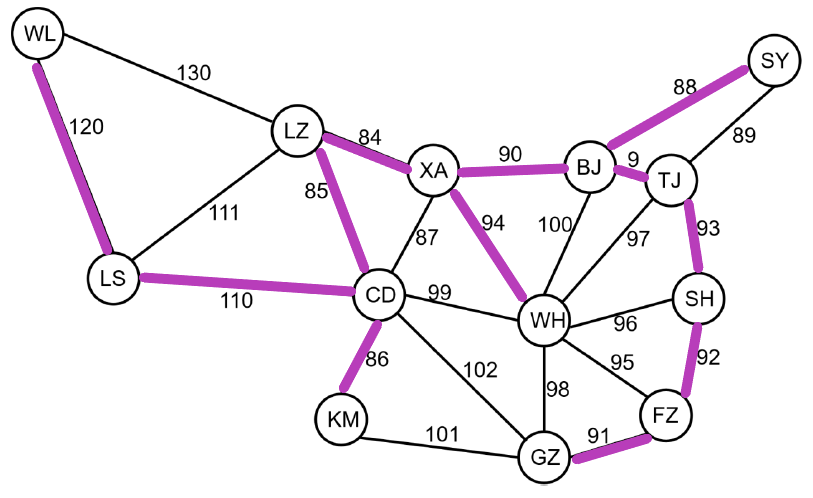
\includegraphics[width=4in]{content/mst.png}


\subsubsection*{e. MST with binary tree}
When \verb|WH| is chosen as the root node, the MST tree can be spanned in this order: \newline
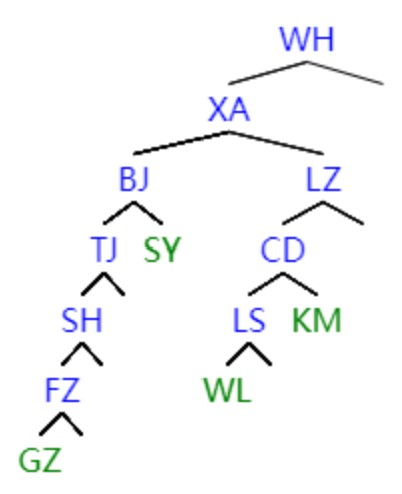
\includegraphics[width=1.5in]{content/bin.jpg}

In this case the MST is a binary tree. 
We give the traverses of this tree:
\begin{itemize}
    \item Preorder: WH - XA - BJ - TJ - SH - FZ - GZ - SY - LZ - CD - LS - WL - KM
    \item Inorder: \ \ GZ - FZ - SH - TJ - BJ - SY - XA - WL - LS - CD - KM - LZ - WH
    \item Postorder: GZ - FZ - SH - TJ - SY - BJ - WL - LS - KM - CD - LZ - XA - WH
\end{itemize}

That's all for \textit{task 3}.
\section{T4}

Realize the minimum distance with Dijkstra's algorithm. The algorithm holds the idea that in a graph where there is no cycle of negative weights, we can recurrently determine the minimum distance from the already-determined nodes.

\subsection{Code Designs}
\subsubsection*{a and b. Implement the generic \textbf{DijkstraAM}}

The only function is \mintinline{c++}{preceding_vertice_map_type dijkstraAM(}\newline
\mintinline{c++}{                  AM am, vertice_type src, vertice_type dst);}\newline
We want to in the meanwhile calculate the minimal distance, and be able to construct the route planned. So the return type of this function is: \newline
\mintinline{c++}{using preceding_vertice_map_type = std::map<vertice_type, vertice_type>;}\newline
which is a map from the current node to its previous one. With this structure we can easily establish the chosen route.

\subsection{QAs}

\subsubsection*{c. Completion of pseudo code of Dijkstra's algorithm}

\begin{algorithm*}  
\caption{Dijkstra's Algorithm}  
% \label{alg:A}  
\begin{algorithmic}  
\STATE {Push the start vertex $S$ into Queue}   
\WHILE{Queue is not empty and the destination vertex $D$ has not been popped}
\STATE Pop the vertex with \boxed{\textsc{\textbf{minimum}}} distance from Queue
\FOR{vertex in the non-traversed neighbors of the popped vertex}
\IF{vertex is not in Queue} \STATE push vertex (with its current distance to $S$) into Queue \ENDIF
\IF{vertex already exists in Queue} \STATE update the distance of vertex in Queue if necessary \ENDIF
\ENDFOR
\ENDWHILE
\end{algorithmic}  
\end{algorithm*}

The required fill in the blank is boxed and emphasized in the pseudo code in next page.

\subsubsection*{d. demonstrate \textbf{DijkstraAM}}
To save space, more details please run the executable under the root working directory with
command: \verb|build/test_dijkstra|. The Extract of the executing procedure and the sorted sequence is: 
\begin{verbatim}
Updating around: SY
turn: 1
Current heap of size: 14
Print current heap's keys:
SY BJ TJ SY GZ FZ SH WL XA LS WH LZ KM CD 
Print current heap's values:
0 88 89 2139062143 2139062143 2139062143 2139062143 2139062143 2139062143 
2139062143 2139062143 2139062143 2139062143 2139062143 
Poping: SY : 0
Updating around: BJ
turn: 2
...
...
...
Updating around: LS
turn: 12
Current heap of size: 3
Print current heap's keys:
LS WL SY 
Print current heap's values:
373 392 2139062143 
Poping: LS : 373
Minimum distance from src: SY, dst: LS >> 373
BJ : SY
CD : XA
FZ : WH
GZ : WH
KM : CD
LS : LZ
LZ : XA
SH : TJ
TJ : SY
WH : TJ
WL : LZ
XA : BJ
LS <- LZ <- XA <- BJ <- SY
\end{verbatim}

The minimal distance from \verb|ST| to \verb|LS| is \boxed{$373$}

That's all for \textit{task 4}.
% \input{content/conclusion}

% \bibliographystyle{plainnat}
% \bibliography{ref}

\newpage
\appendix
\section{How to \emph{reproduce} all the results in this report}

Please refer to the \verb|README.md| in the root directory of the codes. You will see the usage of \verb|make|, which helps you how to establish the same working environment and then to execute and also there are other functions. 

\end{document}